%% ma: L12-B01-0012
%% lop: 12
%% chuong: 1
%% bai: 1
%% dang: 12.1.3
%% loai: TN4
%% muc: TH
%% dap_an: "B"
%% nguon: "(NBV)-ĐỀ SỐ 8-MỖI NGÀY 1 ĐỀ THI 2025.pdf (D08, MỖI NGÀY 1 ĐỀ - Đề số 8), Phần I Câu 1"
%% kien_thuc: "Bài 1 (tính đơn điệu của hàm số, đọc từ bảng biến thiên)"
%% trang_thai: cho-duyet
%% ly_do: "Phương án nhiễu D ('nghịch biến với mọi x ≠ 3') diễn đạt không chuẩn: tính đơn điệu là tính chất trên khoảng, nên D có thể bị hiểu là đúng (f'(x) < 0 với mọi x ≠ 3). TN4 cần đúng 1 phương án đúng."
%% ghi_chu: "Bảng biến thiên vẽ lại bằng tkz-tab theo hình gốc. Đáp án gốc B đúng. Gợi ý sửa D thành 'Hàm số nghịch biến trên khoảng (2;4)' (sai rõ ràng) hoặc bỏ D. Cùng ý tưởng với các câu dạng 12.1.3."
\begin{ex}
Cho hàm số $y=f(x)$ xác định trên $\mathbb R\setminus\{3\}$, liên tục trên mỗi khoảng xác định và có bảng biến thiên như sau:
\begin{center}
\begin{tikzpicture}
  \tkzTabInit[lgt=1.4,espcl=3.2]{$x$/.8,$f'(x)$/.8,$f(x)$/2}{$-\infty$,$3$,$+\infty$}
  \tkzTabLine{,-,d,-,}
  \tkzTabVar{+/$2$,-D+/$-\infty$/$+\infty$,-/$2$}
\end{tikzpicture}
\end{center}
Khẳng định nào sau đây đúng?
\choice{Hàm số nghịch biến trên $\mathbb R\setminus\{3\}$}{\True Hàm số nghịch biến trên mỗi khoảng $(-\infty;3)$ và $(3;+\infty)$}{Hàm số đồng biến trên mỗi khoảng $(-\infty;3)$ và $(3;+\infty)$}{Hàm số nghịch biến với mọi $x\ne3$}
\loigiai{Từ bảng biến thiên, $f'(x)<0$ với mọi $x\ne3$ nên hàm số nghịch biến trên mỗi khoảng $(-\infty;3)$ và $(3;+\infty)$. Phương án A sai vì hàm số gián đoạn tại $x=3$: với $x_1<3<x_2$ thì $f(x_1)<2<f(x_2)$ (nhánh trái nhận giá trị nhỏ hơn $2$, nhánh phải nhận giá trị lớn hơn $2$), nên hàm số không nghịch biến trên cả tập $\mathbb R\setminus\{3\}$. Phương án C sai vì $f'(x)<0$.}
\end{ex}
